\newcommand{\mbf}[1]{\ensuremath\mathbf{#1}}
\def\i{\mbf{\kern1pti\kern1pt}}
\section{Wechselstromkreise}
\subsection{Grundlagen}
Im folgenden werden wir uns mit Wechselstromkreisen aus idealen \emph{passiven Bauelementen} beschäftigen, welche
Widerstand, Spule und Kondensator sind. Diese Elemente werden als \emph{passiv} bezeichnet, da sie kein Signal
verstärken können.

Im Gegensatz zu Gleichstromkreisen beschränken wir uns auf Spannungs- und Stromquellen, welche sinusförmige Signale über
die Zeit der Form
\begin{equation}\label{eq:sinusform}
    U(t) = \hat U\sin(\omega t + \phi_{0/U}) \qquad
    I(t) = \hat I\sin(\omega t + \phi_{0/I})
\end{equation}
erzeugen. Hier ist $\hat U, \hat I$ die \emph{Amplitude}, $\phi_0$ die \emph{Phase} und  $\omega$ die sogenannte
\emph{Kreisfrequenz}. Die Periodendauer $T$ ergibt sich aus der Frequenz $f = \omega/2\pi$ als $T = 1/f = 2\pi/\omega$.
Im folgenden wird die Kreisfrequenz $\omega$ beliebig aber fest sein.

Diese Einschränkungen scheinen zunächst sehr limitiert, doch es wird sich durch diese Annahmen offenbaren, wie sich die
scheinbar verschiedenen Bauteile sich mathematisch vereinen lassen. Dieses schöne und anschauliche Modell legt die
Grundlage für viele komplexere Themen der Elektronik. Wir hoffen mit unserem Kurs einen Einblick und vor allem eine
Intuition für Wechselstromkreise zu schaffen, welche die unterliegende Struktur offenbart.

\subsection{Die Bauteile}
Jedes der drei Bauteile ist symmetrisch und besitzt zwei Kontakte. Die \emph{Spannung} $U$ über dem Bauteil ist die
elektrische Potentialdifferenz zwischen beiden Kontakten. Man sagt, dass die Spannung $U$ \emph{über dem Bauteil
abfällt}. Der Strom $I$ fließt durch das Bauteil von einem in den anderen Kontakt -- dabei muss jedoch eine Richtung
gewählt werden, damit das Vorzeichen eindeutig ist.

Die Spannung ist die Potentialdifferenz $U = \oldphi_2 - \oldphi_1$ von einem zum anderen Kontakt. Als Konvention wird der
Strom wird immer so angegeben, dass die positive Richtung von Kontakt 2 zu Kontakt 1 fließt. Man kann sich an Hand des
ohmschen Widerstands im Gleichstromkreis merken, dass der positive Strom vom höheren zum niedrigeren Potential fließt.

Jedes Bauteil besitzt eine eigene Kenngröße, welche das Verhalten und $U$ und $I$ und somit das Bauelement selbst
vollständig charakterisiert. Wir nehmen alle Bauteile als ideal an, und gehen nicht auf den Aufbau ein.

\paragraph*{Der Widerstand} folgt dem ohmschen Gesetz
\begin{equation}\label{eq:R}
    U = R\cdot I ~.
\end{equation}
Strom und Spannung sind proportional. Die Kenngröße $R$ wird ebenfalls als \emph{Widerstand} bezeichnet und in Ohm
($\si{\ohm} = \si{V}/\si{A}$) angegeben. Ein Widerstand wandelt elektrische Leistung in Wärmeleistung um.
\begin{figure}[H]
    \centering
    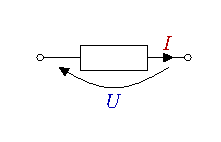
\includegraphics[width=0.3\textwidth]{kBR.pdf}
    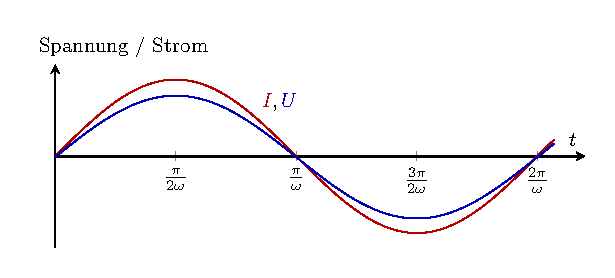
\includegraphics[width=0.6\textwidth]{kPR.pdf}
    \caption{Das Widerstandsschaltsymbol und dessen $U(t),\, I(t)$ Relation}
\end{figure}

\paragraph*{Der Kondensator}
folgt der Gleichung
\begin{equation}\label{eq:C}
    I = C\,\dv{U}{t} ~.
\end{equation}
Der Strom ist proportional zur zeitlichen Änderung der Spannung. Die Größe $C$ wird als \emph{Kapazität} bezeichnet und
in Farad ($\si{\farad} = \si{\ampere\second}/\si{\volt}$) angegeben. Häufig wird der Kondensator als Ladungsspeicher $Q
= CU$ eingeführt, aber dies ist irreführend: Die Gesamtladung eines Kondensators ist immer 0, da der gleiche Strom ein-
wie ausfließt. Stattdessen speichert der Kondensator elektrische Energie in seinem elektrischen Feld. Im Bild der
Wechselstromkreise ist die Anschauung hilfreich, dass ein Kondensator Änderungen der Spannung durch Strom entgegenwirkt.
\begin{figure}[H]
    \centering
    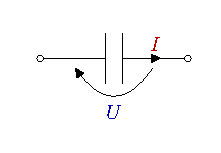
\includegraphics[width=0.3\textwidth]{kBC.pdf}
    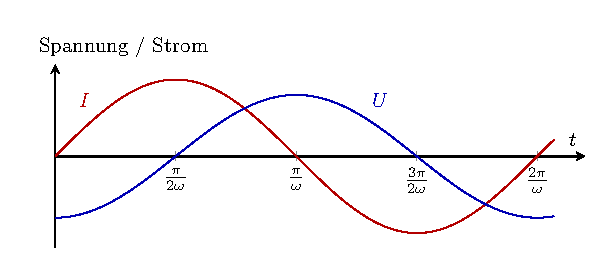
\includegraphics[width=0.6\textwidth]{kPC.pdf}
    \caption{Das Kondensatorschaltsymbol und dessen $U(t),\, I(t)$ Relation}
\end{figure}

\paragraph*{Die Spule}
ist das Gegenbild des Kondensators und folgt nach Selbstinduktion der Gleichung
\begin{equation}\label{eq:L}
    U = L\,\dv{I}{t} ~.
\end{equation}
Die Spannung ist proportional und entgegengesetzt zur Änderung des Stroms. Die Größe $L$ ist die \emph{Induktivität} und
wird in Henry ($\si{\henry} = \si{\volt\second}/\si{\ampere}$) angegeben. Eine Spule speichert elektrische Energie in
ihrem Magnetfeld. Man kann sich merken, dass eine Spule Änderungen im Strom durch eine induzierte Spannung
entgegenwirkt.
\begin{figure}[H]
    \centering
    \includegraphics[width=0.3\textwidth]{kBL.pdf}
    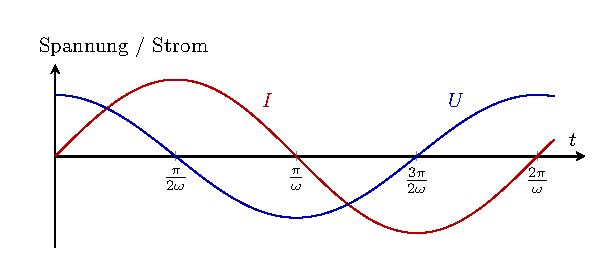
\includegraphics[width=0.6\textwidth]{kPL.pdf}
    \caption{Das Spulenschaltsymbol und dessen $U(t),\, I(t)$ Relation}
\end{figure}

\subsection{Linearität}
Diese drei Komponenten mögen zunächst sehr verschieden wirken, jedoch sind sie durch zwei Eigenschaften vereint, welche
sich später als sehr nützlich erweisen werden: Sie verhalten sich \emph{linear} und \emph{zeitinvariant}. Um dies zu
verstehen, müssen die Gleichungen \eqref{eq:R}, \eqref{eq:C}, \eqref{eq:L} als Bedingung zwischen einem zeitlichen
Verlauf von $U(t)$ und $I(t)$ gesehen werden.

\def\llra{~\longleftrightarrow~}
Man betrachte also ein beliebiges der drei Bauteile, sowie einen Verlauf $U(t)$ und $I(t)$, welche die charakteristische
Gleichung erfüllen. Wir kürzen dies als
$$U(t) \llra I(t)$$
ab. Damit drücken wir also aus, dass der Verlauf $U(t)$ links mit dem Verlauf $I(t)$ rechts diesem bestimmten Bauteil
genügt.
Ist dies der Fall, so folgt:
\begin{enumerate}[label=(\arabic*)]
    \item
        \[ a\cdot U(t) \llra a \cdot I(t) \]
        erfüllt ebenfalls die Gleichung, wobei $a$ ein beliebiger Faktor ist.
    \item Gilt
        \[ U_1(t) \llra I_1(t) \qquad U_2(t) \llra I_2(t) ~,\]
        so folgt
        \[ U_1(t) + U_2(t) \llra I_1(t) + I_2(t) ~. \]
    \item Es gilt
        \[ U(t+\tau) \llra I(t+\tau) \]
        für alle Zeitverschiebungen $\tau$.
\end{enumerate}

Es lässt sich schnell überprüfen, dass diese Eigenschaften von allen drei Bauteilen erfüllt werden: Ableitungen sowie
Skalarmultiplikation sind linear, und keine der charakteristischen Gleichungen enthält eine explizite Zeitabhängigkeit.
\\

Was bedeuten diese Eigenschaften für unsere sinusförmigen Strom- und Spannung-Verläufe? Zunächst lässt sich aus der
Zeitinvarianz folgern, dass wenn $U$ oder $I$ periodisch sind, das jeweils andere auch periodisch sein muss: Verschiebt
man beide um sie Periodendauer $T$, so sieht das periodische genau so aus wie vorher -- also muss die um $T$ verschobene
andere Größe ebenfalls gleich bleiben. Damit ist sie periodisch.

Zudem sagt uns Zeitinvarianz, dass die absolute Phase $\phi_0$ eines Signals gemäß \eqref{eq:sinusform} irrelevant ist,
da ich sie mit $\tau = -\phi_0$ verschwinden lassen kann; nur die relative Phase $\phi$ zwischen $U(t)$ und $I(t)$
bleibt.

Setzt man für alle drei Bauteile sinusförmige Wellenformen ein, so erhält man folgende Lösungen (Im Kopf, Ableiten vom
Sinus ist eine Verschiebung um $\pi/2$ !).
\begin{align*}
    \text{Widerstand} &: & \underbrace{R\cdot \hat I}_{\hat U}\sin(\omega t)
    & \llra \hat{I}\sin(\omega t)
    \\
    \text{Kondensator} &: & \hat U\sin(\omega t)
    & \llra \underbrace{\omega C \cdot \hat U}_{\hat{I}}\sin(\omega t + \pi/2)
    \\
\text{Spule} &: &  \underbrace{\omega L\cdot \hat I}_{\hat U}\sin(\omega t + \pi/2)
    & \llra \hat{I}\sin(\omega t)
\end{align*}
Mittels den Eigenschaften der Linearität und Zeitinvarianz können wir dies in eine einheitliche Form bringen, indem wir
die Rechte Seite zu $I(t) = \hat I\sin(\omega t)$ umformen.
\begin{gather}\label{eq:RLC}
\begin{aligned}
    \text{Widerstand} &: & U(t) = R \cdot \hat I\sin(\omega t)
    & \llra \hat{I}\sin(\omega t)
    \\
    \text{Kondensator} &: & U(t) = {1\over \omega C}\cdot  \hat I\sin(\omega t - \pi/2)
    & \llra \hat{I}\sin(\omega t)
    \\
\text{Spule} &: &  U(t) = \omega L \cdot \hat I\sin(\omega t + \pi/2)
    & \llra \hat{I}\sin(\omega t)
\end{aligned}
\end{gather}
Jedes der Bauteile lässt sich im Wechselstromkreis einer festen Kreisfrequenz $\omega$ also allein durch einen
bestimmten Absolutbetrag $\hat U / \hat I$ sowie einer Phasenverschiebung $\phi$ darstellen.
\begin{center}
    \begin{tabular}{rcc}
        Bauteil & $\hat U / \hat I$ & $\phi$ \\
        \hline
        Widerstand & $R$ & 0 \\
        Kondensator & ${1/\omega C}$ & $-\pi/2$ \\
        Spule & $\omega L$ & $\pi/2$
    \end{tabular}
\end{center}

Weiterhin wissen wir so, dass beliebige Spannungs- und Stromverläufe $U(t), I(t)$ innerhalb jedes Wechselstromkreises
sinusförmig mit gleicher Kreisfrequenz $\omega$ sein müssen, da jedes Bauteil die Sinusform erhält und lineare
Kombinationen von Sinen ebenfalls eine Sinusform gleicher Frequenz ergeben. Demnach sind in einem Wechselstromkreis
fester Kreisfrequenz $\omega$ ebenfalls jegliche Strom- und Spannungsformen ausgezeichnet durch einen Betrag (die
Amplitude) und einer Phase (welche sich auf eine beliebige Bezugswellenform bezieht, nach Zeitinvarianz).

\subsection{Mathematische Darstellung}
\subsubsection{Zeigerdiagramme}
Zusammenfassend haben wir im vorherigen Abschnitt erkannt, dass das Verhalten jedes der drei Bauteile sich durch einen
absoluten Wert und eine Phase darstellen lässt, ebenso wie jegliche Ströme und Spannungen. Wir suchen also nach einer
Möglichkeit, all diese Dinge in einem mathematischen Konzept zu vereinen.

Der Sinus stammt aus dem Kreis -- nimmt man eine Komponente einer Kreisbewegung entlang des Einheitskreises in der
Ebene, so erhält man eine sinusförmige Funktion.
\begin{figure}[H]
    \centering
    \begin{tikzpicture}
        \coordinate (M) at (-3, 0);
        \path (M) -- ++(60:2) node[inner sep=1pt] (P) {};

        \draw[thick, ->] (0, 0) -- (9, 0) node[right] {$t$};
        \draw[thick, ->] (0, 0) -- +(0, 2.2);
        \draw[thick, ->] (M) -- +(2.2, 0);
        \draw[thick, ->] (M) -- +(0, 2.2);

        \draw (0, 0) sin (2, 2) cos (4, 0)
            (8, 0) sin (6, -2) cos (4, 0);

        \draw (M) circle (2);
        \draw[dashed] (P)++(-1, 0) -- (1.333, 1.732);

        \draw[very thick, red, -{Latex[flex=0]}] (-1, 0) arc (0:60:2);
        \draw[very thick, black, -{Latex}] (M) -- (P);

        \draw[very thick, blue] (-2, 0) -- (P)
            (1.333, 0) -- +(0, 1.732);
        \draw[very thick, red] (0, 0) -- node[below,red] {$t$} (1.333, 0);

        \node[draw,red,shape=circle,fill=red,inner sep=1pt] at (P) {};

        \path (M) -- ++(30:2.5) node[red] {$\omega t$};
    \end{tikzpicture}
    \caption{Sinuskurve als Komponente der Kreisbewegung}
\end{figure}
Betrachten also die Größen als \emph{Zeiger} vom Ursprung, welche einen Betrag $A$ und einen Winkel $\phi$ zur $x$-Achse
besitzen.  Der Wert der Größe zu jedem Zeitpunkt ist seine $x$-Komponente. Lassen wir nun den Zeiger mit einer
Kreisfrequenz $\omega$ um den Ursprung drehen, sodass zu Zeitpunkt $t$ das Zeigerdiagramm um den Winkel $\omega t$ aus
der Ausgangslage gedreht ist. Dann wird der Wert genau einer sinusförmigen Funktion mit Phase $\phi$
und Amplitude $A$ folgen. In dieser Darstellung können wir also jeder sinusförmigen Funktion eindeutig einen Zeiger in
der Ebene zuordnen.

\begin{figure}[H]
    \centering
    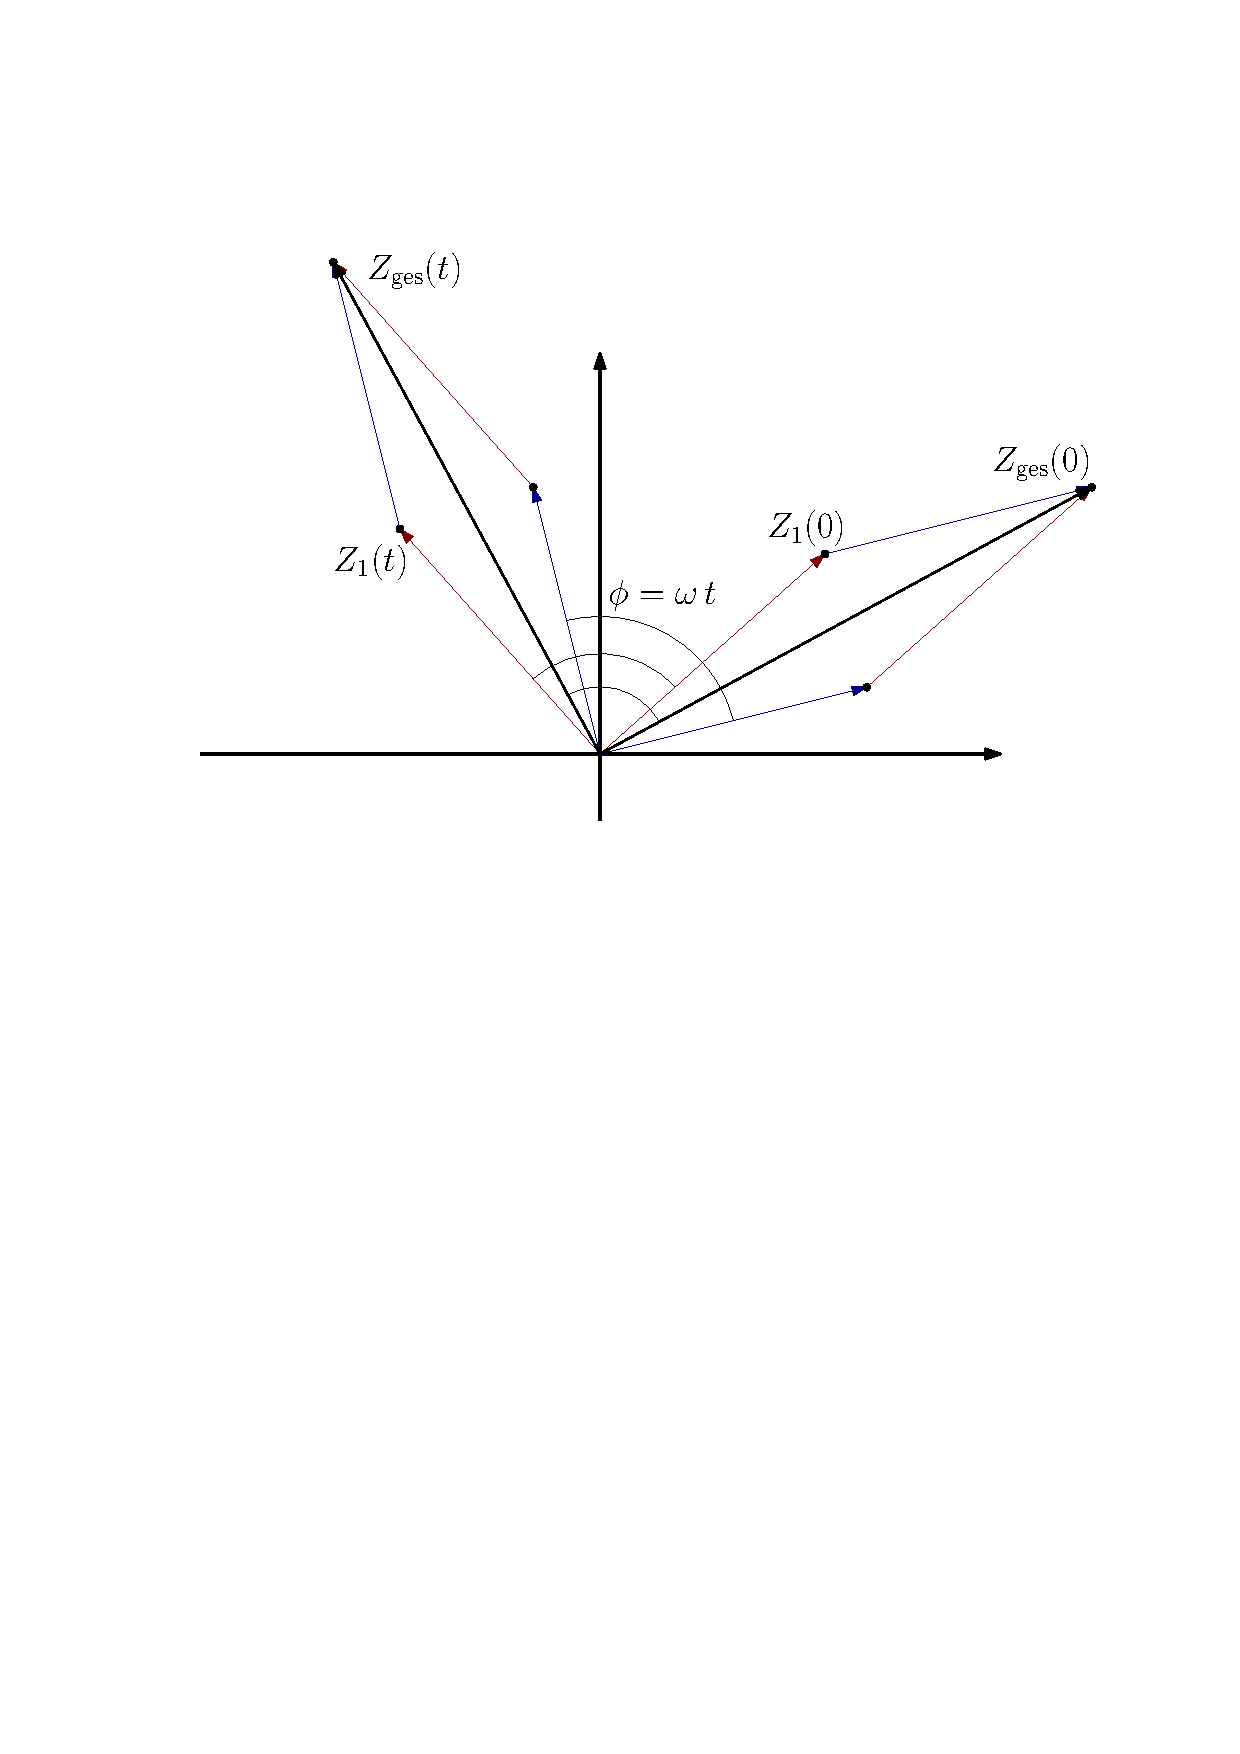
\includegraphics[width=.7\textwidth]{kZeiger.pdf}
    \caption{Vektoraddition im Zeigerdiagramm}
\end{figure}

Addiert man zwei Zeiger gemäß der Vektoraddition, addieren sich ebenfalls die $x$-Komponenten. Man bemerke, dass es egal
ist, zuerst die Zeiger zu addieren, und dann das Ergebnis um einen Winkel $\omega t$ zu drehen, oder umgekehrt. Dank
Zeitinvarianz können wir die Zeiger zum Zeitpunkt $t = 0$ addieren, und erhalten sofort den Zeiger, der der Wellenform
der Summe der beiden anderen Wellenformen entspricht.

Es wird sichtbar, dass unsere Bauteile sehr ähnlich sind: Legen wir eine Spannungswellenform an, so stehen die
Stromzeiger von Kondensator und Spule im rechten Winkel auf dem Spannungszeiger, während der Widerstand in die selbe
Richtung zeigt.




\subsubsection{Komplexe Darstellung}
Diese Darstellung ermöglicht es uns also, Strom- und Spannungskurven geometrisch zu interpretieren. Jedoch würden wir gerne
algebraisch rechnen können, um konkrete Werte auszurechnen.

%Insbesondere suchen wir eine Möglichkeit, den Begriff des Widerstandes auf eine Relation zwischen Strom und Spannung
%eines Bauteils im Wechselstromkreis zu verallgemeinern.

Dazu führen wir \emph{Komplexe Zahlen} ein. Komplexe Zahlen spannen im Gegensatz zu Reellen Zahlen keine Zahlengerade,
sondern die Ebene auf. Jede Komplexe Zahl $z = a+b\i$ besteht aus zwei Teilen: dem \emph{Realteil} $a$ und dem
\emph{Imaginärteil} $b$. Die Konstante $i$ ist die Imaginäre Einheit, und ist definiert über $i^2 = -1$. Alleine diese
Eigenschaften reichen aus, um das Rechnen mit Komplexen Zahlen vollständig zu beschreiben.

Wir ersetzen also die Zeiger mit der entsprechenden komplexen Zahl, sodass die $x$-Komponente der Realteil und die
$y$-Komponente der Imaginärteil ist. Komplexe Zahlen addieren sich ebenfalls komponentenweise, sodass die Vektoraddition
erhalten bleibt. Die wahre Macht dieser scheinbar umständlichen Definition findet sich aber erst in der Euler'schen
Formel:
\begin{equation}\label{eq:euler}
    e^{i\phi} = \cos \phi + i\sin \phi
\end{equation}
Wow! Was sagt uns das? Die komplexe Zahl $e^{i\phi}$ liegt auf dem Einheitskreis und hat den Winkel $\phi$ zur reellen
Achse -- also die Phase! Multiplizieren wir mit einem positiven reellen Betrag $A$, so können wir jede komplexe Zahl direkt
aus Betrag und Winkel darstellen. Dies nennt man die polare Darstellung.
\begin{equation}\label{eq:polar}
    Ae^{i\phi} = A(\cos \phi + i\sin \phi)
\end{equation}
Aus dieser Darstellung können wir über die Rechenregeln der Exponentialfunktion direkt die Multiplikation von komplexen
Zahlen verstehen:
\[ Ae^{i\phi} \cdot Be^{i\psi} = ABe^{i(\phi+\psi)} \]
Die Beträge multiplizieren sich, die Phasen addieren sich. Eine andere Weise dies zu betrachten ist, dass die
Multiplikation mit einer Zahl $Ae^{i\phi}$ die Ebene um einen Faktor $A$ streckt, und um einen Winkel $\phi$ dreht.

Letzteres können wir gebrauchen: Um das Zeigerdiagramm zum Zeitpunkt $t$ zu bekommen, muss der Ausgangszustand zu $t=0$
um den Winkel $\omega t$ gedreht werden -- also mit $e^{i\omega t}$ multipliziert. Damit lautet die Zeitentwicklung
einer komplexen Größe $\mbf z$
\begin{equation}
    \mbf z\cdot e^{i\omega t}
\end{equation}
Wenn wir $\mbf z$ polar darstellen als $\mbf z = \hat A e^{i\phi}$ mit Betrag (Amplitude) $\hat A$ und Winkel (Phase) $\phi$, erkennen wir
etwas wieder

\begin{gather*}
    \Re\qty(\mbf z\cdot e^{i\omega t})
    = \Re\qty(\hat Ae^{i\phi} \cdot e^{i\omega t})
    = \Re\qty(\hat Ae^{i(\omega t + \phi)})
    = \hat A\Re\qty(\cos(\omega t + \phi) + i\sin(\omega t + \phi)) \\
    = \hat A\cos(\omega t  +\phi)
    = \hat A\sin(\omega t + \phi + \pi/2)
\end{gather*}
Der Realteil entspricht genau einer Sinusform mit Amplitude $A$ und Phasenverschiebung $\phi+\pi/2$. Dank Zeitinvarianz
ist die Konstante Phase $\pi/2$ allerdings irrelevant, da man wie bereits gesagt nur Phasen zwischen Größen
vergleicht.\footnote{Die Wahl des Realteils ist auch Konvention. Man hätte genau so gut den Imaginärteil nehmen können,
was einem die Phase erspart hätte.}
\subsection{Impedanz}
Wir hatten zuvor gesehen, dass sich die Relation von $U(t)$ und $I(t)$ für ein gegebenes Bauteil durch ein Verhältnis
der Amplituden sowie einer Phasendifferenz beschreiben lässt. Zudem hatten wir erkannt, dass diese Relation linear ist.

Der komplexe Zahlenraum ermöglicht es uns, dies in einer einzigen komplexen Zahl zusammenzufassen: Wir definieren die
\emph{Impedanz} $\mbf Z$ eines Bauteils so, dass für die komplexe Darstellung von Strom $\mbf I$ und Spannung $\mbf U$
\begin{equation}\label{eq:impedanz}
    \mbf U = \mbf Z \cdot \mbf I
\end{equation}
Dies sieht dem Ohmschen Gesetz \eqref{eq:R} sehr ähnlich, jedoch ist jede Größe komplex. Die Impedanz enthält sowohl
einen Betrag als auch eine Phase. Diese Phase stellt nach komplexer Multiplikation genau die Phasendifferenz zwischen
$\mbf U$ und $\mbf I$ dar. Die Linearität der Bauteile äußert sich also direkt als lineare Gleichung -- im Komplexen.

Für den Widerstand bleibt die Impedanz $\mbf Z = R$ reell. Die Spule und der Kondensator weisen jeweils eine
Phasenverschiebung von $\pm \pi/2$ auf. Das entspricht einem Faktor von $e^{\pm i\pi/2}= \pm i$. Drücken wir also die
Ergebnisse aus \eqref{eq:RLC} in Form komplexer Impedanzen aus, erhalten wir:
\begin{align}
    \mbf Z_R &= R \\
    \mbf Z_C &= -\frac i{\omega C} \\
    \mbf Z_L &= i\omega L
\end{align}
Die Impedanz ist die komplexe Erweiterung des Widerstandes, und ähnlich wie sie dem ohmschen Gesetz für den Widerstand
genügt, erfüllt sie auch die Differentialgleichungen \eqref{eq:C}, \eqref{eq:L} für Spule und Widerstand. Zwar sind
diese Gleichungen eigentlich für reellwertige Größen, aber Zeitableitungen agieren einzeln auf Realteil und
Imaginärteil; Wie wir zuvor Zeiger addiert und dann gedreht haben, können wir auch komplexe Größen ableiten und dann den
Realteil nehmen. Setzen wir die komplexe Zeitenwicklung für die jeweiligen Größen ein, zeigt sich:
\begin{gather*}
    \begin{aligned}
        \mbf Ie^{i\omega t} &= C\dv{t}(\mbf Ue^{i\omega t}) \\
        \mbf I &= i\omega C \cdot \mbf U \\
        \mbf U &= - \frac{i}{\omega C} \cdot \mbf I
    \end{aligned}
    \qquad
    \begin{aligned}
        \mbf Ue^{i\omega t} &= L\dv{t}(\mbf Ie^{i\omega t}) \\
        \mbf U &= i\omega L \cdot \mbf I
    \end{aligned}
\end{gather*}

Wir können die imaginären Impedanzen von $L$ und $C$ im Zeigerdiagramm wiederfinden: Sie sind beide
rein imaginär und besitzen $\pi/2$ Phasenverschiebung. Zudem sind sie entgegengesetzt.
\begin{figure}[H]
    \centering
    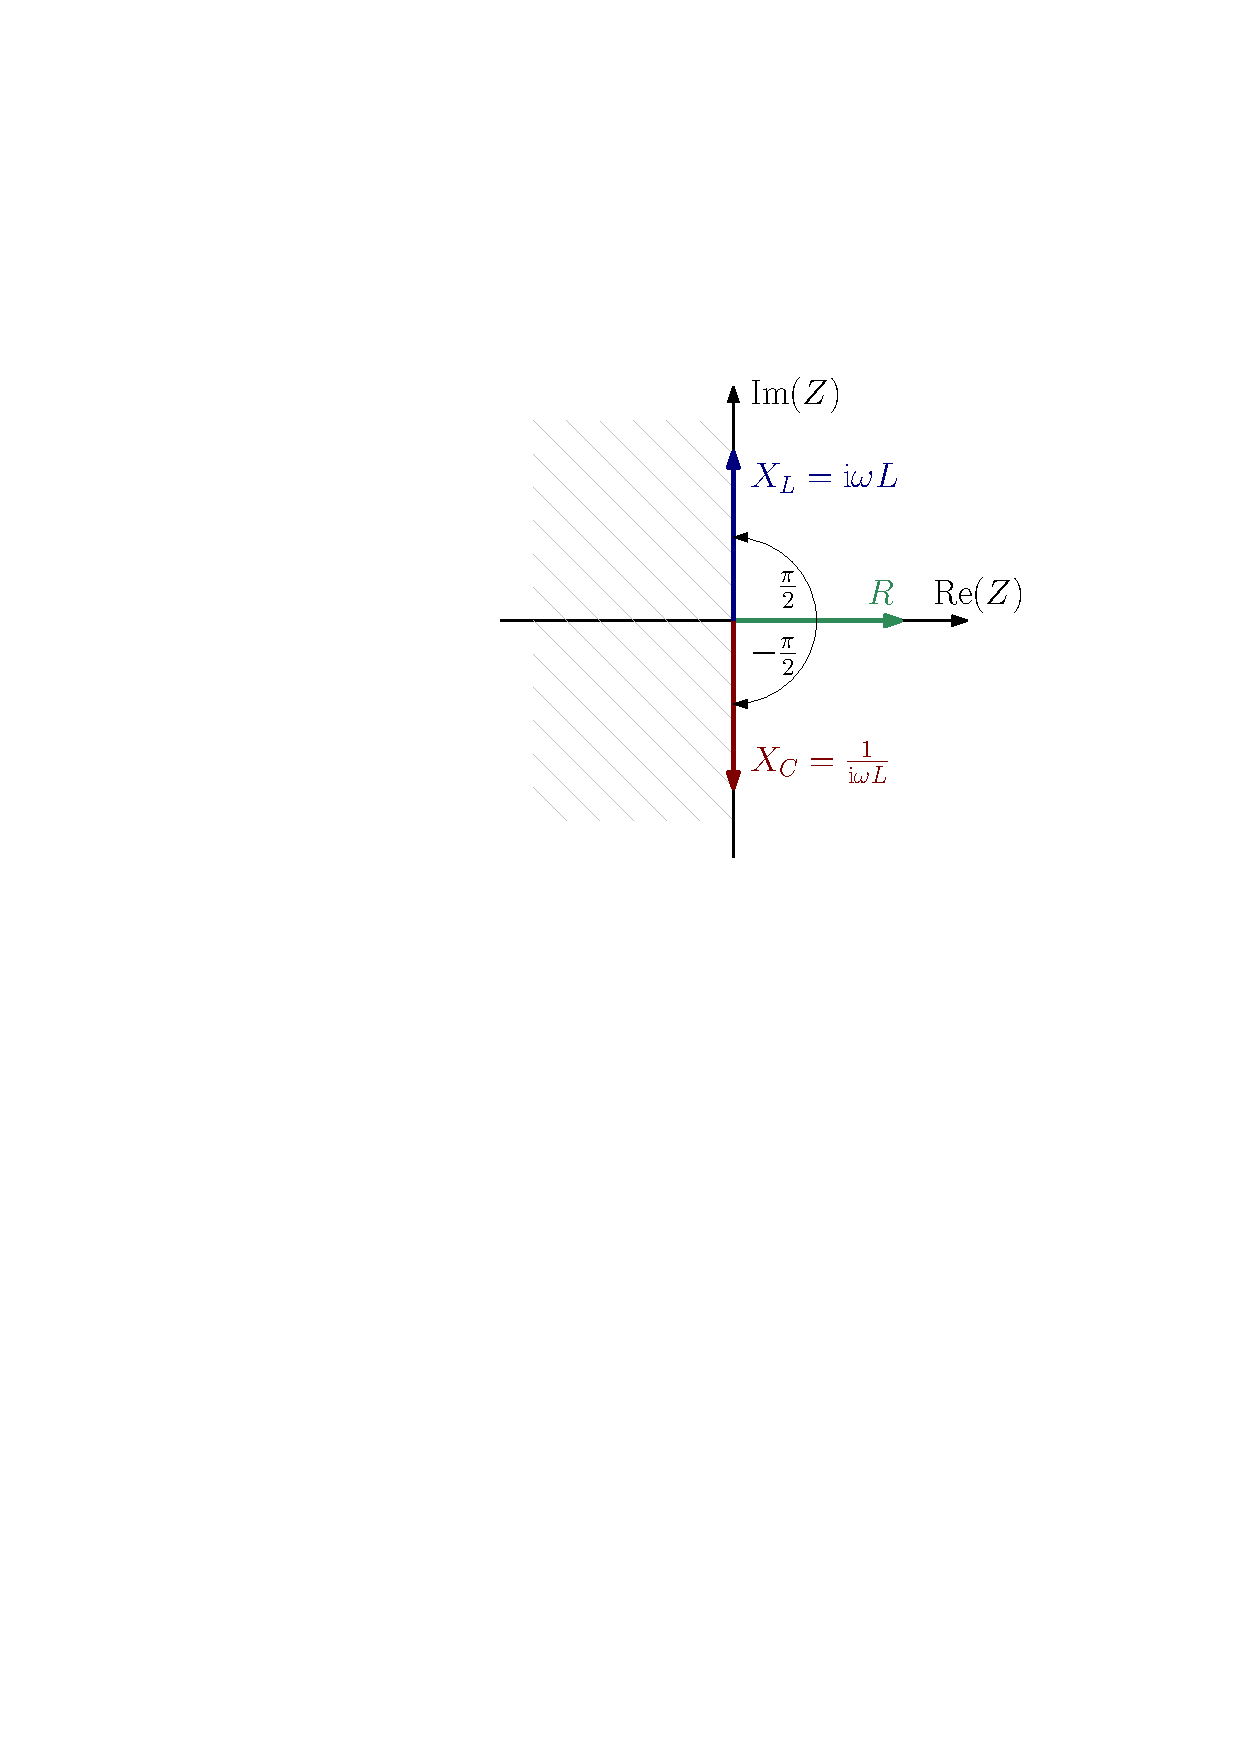
\includegraphics[width=0.5\textwidth]{kCompZeiger.pdf}
    \caption{Bauteilimpedanzen als Zeiger im komplexen Zeigerdiagramm}
\end{figure}
Die komplexen Impedanzen geben uns die Möglichkeit, die geometrische Anschauung mit algebraischer Eleganz zu vereinen.
Damit haben wir die allgemeine Relation zwischen $U(t)$ und $I(t)$
\[ U(T) \llra I(t) \]
, welche wir vorher holprig über Phasenverschiebung
und Amplitudenverhältnis ausdrücken mussten, ersetzt durch eine direkte Proportionalität im komplexen Raum
\[ \mbf U = \mbf Z \cdot \mbf I \]
Um zu unterstreichen, dass es sich um das selbe Konzept handelt, können wir die Impedanz auf die zuvor eingeführten
Eigenschaften der Linearität und Zeitinvarianz testen:
Angenommen die Proportionalität $ \mbf U_{1,2} = \mbf Z \cdot \mbf I_{1,2}$ gilt, dann folgt
\begin{enumerate}[label=(\arabic*)]
    \item
        \[ a\mbf U_1 = a\mbf Z \cdot \mbf I_1 \]
    \item
        \[ \mbf U_1 + \mbf U_2 = \mbf Z \cdot (\mbf I_1 + \mbf I_2) \]
    \item für eine beliebige Zeitverschiebung $\tau$ nach der Zeitenwicklung $e^{i\omega\tau}$
        \[ e^{i\omega\tau}\mbf U_1 = e^{i\omega\tau}\mbf Z \cdot \mbf I_1 ~. \]
\end{enumerate}
Es handelt sich also in der Tat um die anfänglich beschiebene Relation in einer algebraischen Darstellung.

% vim:tw=120
